% $Header: /u/gcmpack/manual/s_algorithm/text/spatial-discrete.tex,v 1.13 2004/03/23 15:29:40 afe Exp $
% $Name:  $

\section{Spatial discretization of the dynamical equations}

Spatial discretization is carried out using the finite volume
method. This amounts to a grid-point method (namely second-order
centered finite difference) in the fluid interior but allows
boundaries to intersect a regular grid allowing a more accurate
representation of the position of the boundary. We treat the
horizontal and vertical directions as separable and differently.

% $Header: /u/gcmpack/manual/s_algorithm/text/notation.tex,v 1.3 2001/08/09 19:24:04 jmc Exp $
% $Name:  $

\section{Notation} 

The notations we use to discribe the discrete formulation 
of the model are summarised hereafter:\\
general notation:
\\ $\Delta x, \Delta y, \Delta r$ grid spacing in X,Y,R directions.
\\ $A_o$ : Area of the face orthogonal to "o" direction (o=u,v,w ...).
\\ ${\cal V}_u , {\cal V}_v , {\cal V}_v , {\cal V}_\theta$ :
Volume of the grid box surrounding $u,v,w,\theta$ point;
\\ $i,j,k$ : current index relative to X,Y,R directions;
\\basic operator:
\\ $\delta_i $ : $\delta_i \Phi = \Phi_{i+1/2} - \Phi_{i-1/2} $
\\ $\overline{~}i$ : $\overline{\Phi}^i = ( \Phi_{i+1/2} + \Phi_{i-1/2} ) / 2 $ 
\\ $\delta_x $ : $\delta_x \Phi = \frac{1}{\Delta x} \delta_i \Phi $
\\
\\ $\overline{\nabla}$ = gradient operator :  
$\overline{\nabla} \Phi = \{ \delta_x \Phi , \delta_y \Phi \}$
\\ $\overline{\nabla} \cdot$ = divergence operator :  
$\overline{\nabla}\cdot \vec{\mathrm{f}}  = 
\frac{1}{\cal A} \{ \delta_i \Delta y \mathrm{f}_x 
                  + \delta_j \Delta x \mathrm{f}_y \} $
\\ $\overline{\nabla}^2 $ = Laplacien operator :
$ \overline{\nabla}^2 \Phi = 
   \overline{\nabla}\cdot \overline{\nabla}\Phi $



\subsection{The finite volume method: finite volumes versus finite difference}
\begin{rawhtml}
<!-- CMIREDIR:finite_volume -->
\end{rawhtml}



The finite volume method is used to discretize the equations in
space. The expression ``finite volume'' actually has two meanings; one
is the method of embedded or intersecting boundaries (shaved or lopped
cells in our terminology) and the other is non-linear interpolation
methods that can deal with non-smooth solutions such as shocks
(i.e. flux limiters for advection). Both make use of the integral form
of the conservation laws to which the {\it weak solution} is a
solution on each finite volume of (sub-domain). The weak solution can
be constructed out of piece-wise constant elements or be
differentiable. The differentiable equations can not be satisfied by
piece-wise constant functions.

As an example, the 1-D constant coefficient advection-diffusion
equation:
\begin{displaymath}
\partial_t \theta + \partial_x ( u \theta - \kappa \partial_x \theta ) = 0
\end{displaymath}
can be discretized by integrating over finite sub-domains, i.e.
the lengths $\Delta x_i$:
\begin{displaymath}
\Delta x \partial_t \theta + \delta_i ( F ) = 0
\end{displaymath}
is exact if $\theta(x)$ is piece-wise constant over the interval
$\Delta x_i$ or more generally if $\theta_i$ is defined as the average
over the interval $\Delta x_i$.

The flux, $F_{i-1/2}$, must be approximated:
\begin{displaymath}
F = u \overline{\theta} - \frac{\kappa}{\Delta x_c} \partial_i \theta
\end{displaymath}
and this is where truncation errors can enter the solution. The
method for obtaining $\overline{\theta}$ is unspecified and a wide
range of possibilities exist including centered and upwind
interpolation, polynomial fits based on the the volume average
definitions of quantities and non-linear interpolation such as
flux-limiters.

Choosing simple centered second-order interpolation and differencing
recovers the same ODE's resulting from finite differencing for the
interior of a fluid. Differences arise at boundaries where a boundary
is not positioned on a regular or smoothly varying grid. This method
is used to represent the topography using lopped cell, see
\cite{adcroft:97}. Subtle difference also appear in more than one
dimension away from boundaries. This happens because the each
direction is discretized independently in the finite difference method
while the integrating over finite volume implicitly treats all
directions simultaneously. Illustration of this is given in
\cite{ac:02}.

\subsection{C grid staggering of variables}

\begin{figure}
\begin{center}
\resizebox{!}{2in}{ 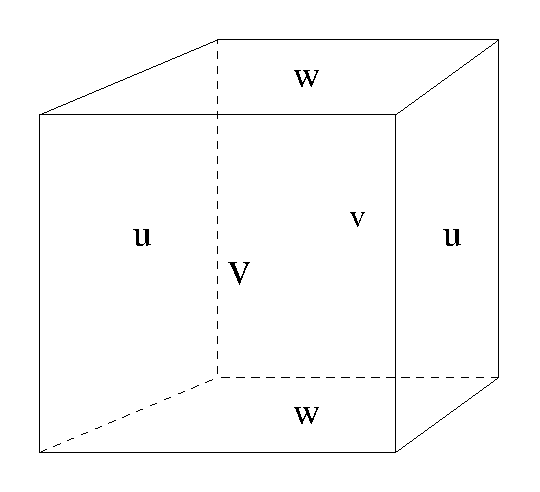
\includegraphics{part2/cgrid3d.eps}}
\end{center}
\caption{Three dimensional staggering of velocity components. This
facilitates the natural discretization of the continuity and tracer
equations. }
\label{fig:cgrid3d}
\end{figure}

The basic algorithm employed for stepping forward the momentum
equations is based on retaining non-divergence of the flow at all
times. This is most naturally done if the components of flow are
staggered in space in the form of an Arakawa C grid \cite{arakawa:77}.

Fig. \ref{fig:cgrid3d} shows the components of flow ($u$,$v$,$w$)
staggered in space such that the zonal component falls on the
interface between continuity cells in the zonal direction. Similarly
for the meridional and vertical directions.  The continuity cell is
synonymous with tracer cells (they are one and the same).



\subsection{Grid initialization and data}

Initialization of grid data is controlled by subroutine {\em
INI\_GRID} which in calls {\em INI\_VERTICAL\_GRID} to initialize the
vertical grid, and then either of {\em INI\_CARTESIAN\_GRID}, {\em
INI\_SPHERICAL\_POLAR\_GRID} or {\em INI\_CURV\-ILINEAR\_GRID} to
initialize the horizontal grid for cartesian, spherical-polar or
curvilinear coordinates respectively.

The reciprocals of all grid quantities are pre-calculated and this is
done in subroutine {\em INI\_MASKS\_ETC} which is called later by
subroutine {\em INITIALIZE\_FIXED}.

All grid descriptors are global arrays and stored in common blocks in
{\em GRID.h} and a generally declared as {\em \_RS}.

\fbox{ \begin{minipage}{4.75in}
{\em S/R INI\_GRID} ({\em model/src/ini\_grid.F})

{\em S/R INI\_MASKS\_ETC} ({\em model/src/ini\_masks\_etc.F})

grid data: ({\em model/inc/GRID.h})
\end{minipage} }


\subsection{Horizontal grid}
\label{sec:spatial_discrete_horizontal_grid}

\begin{figure}
\begin{center}
\begin{tabular}{cc}
  \raisebox{1.5in}{a)}\resizebox{!}{2in}{ 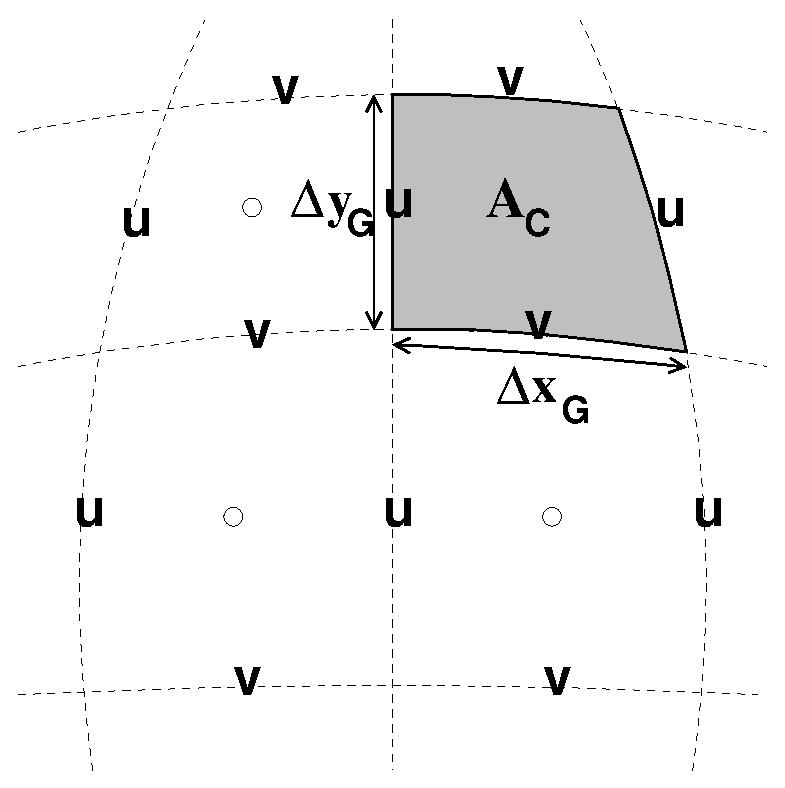
\includegraphics{part2/hgrid-Ac.eps}}
& \raisebox{1.5in}{b)}\resizebox{!}{2in}{ 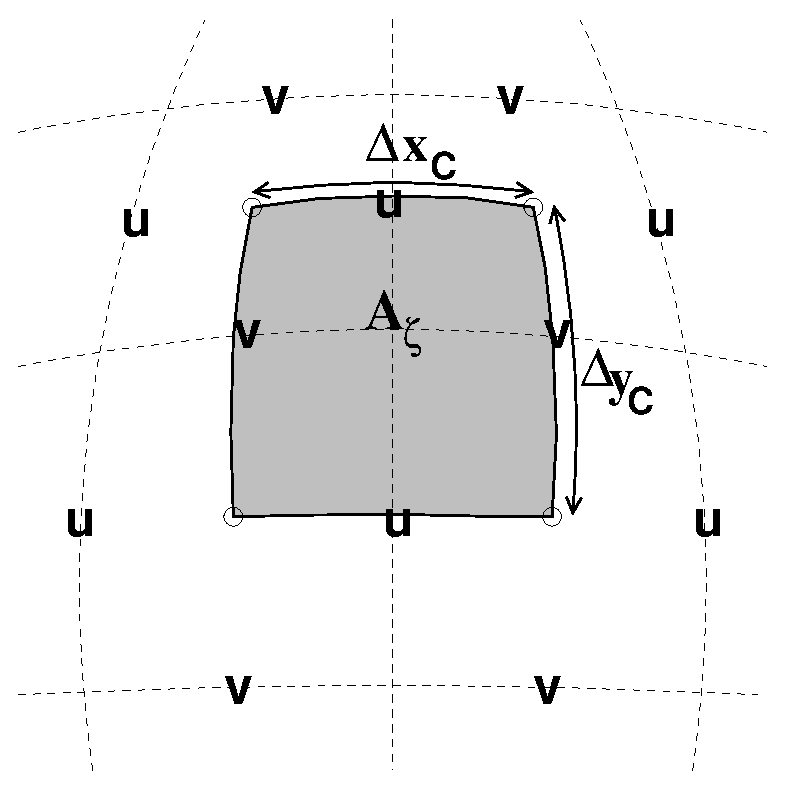
\includegraphics{part2/hgrid-Az.eps}}
\\
  \raisebox{1.5in}{c)}\resizebox{!}{2in}{ 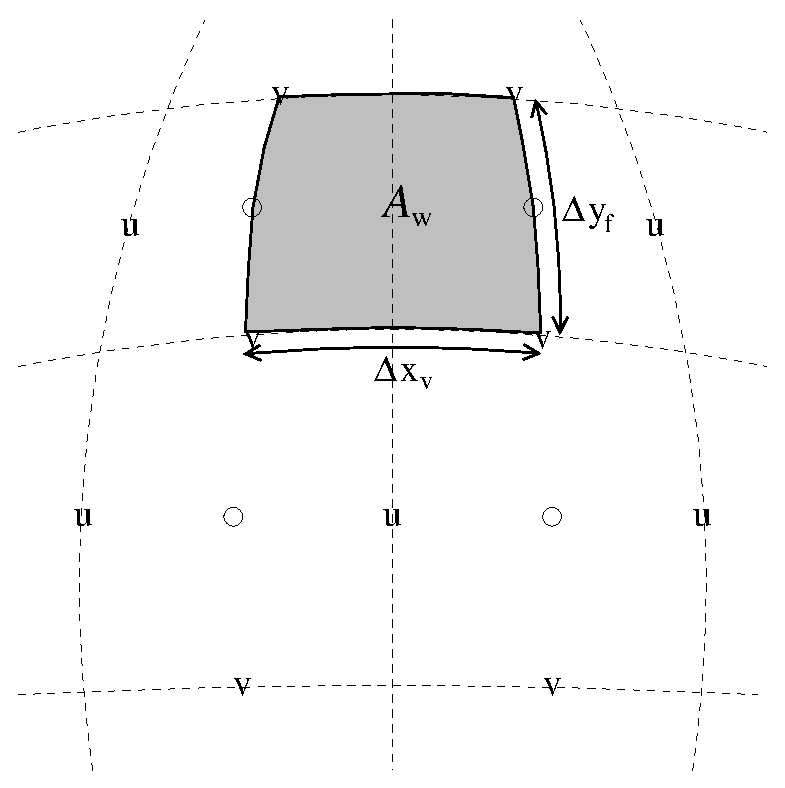
\includegraphics{part2/hgrid-Au.eps}}
& \raisebox{1.5in}{d)}\resizebox{!}{2in}{ 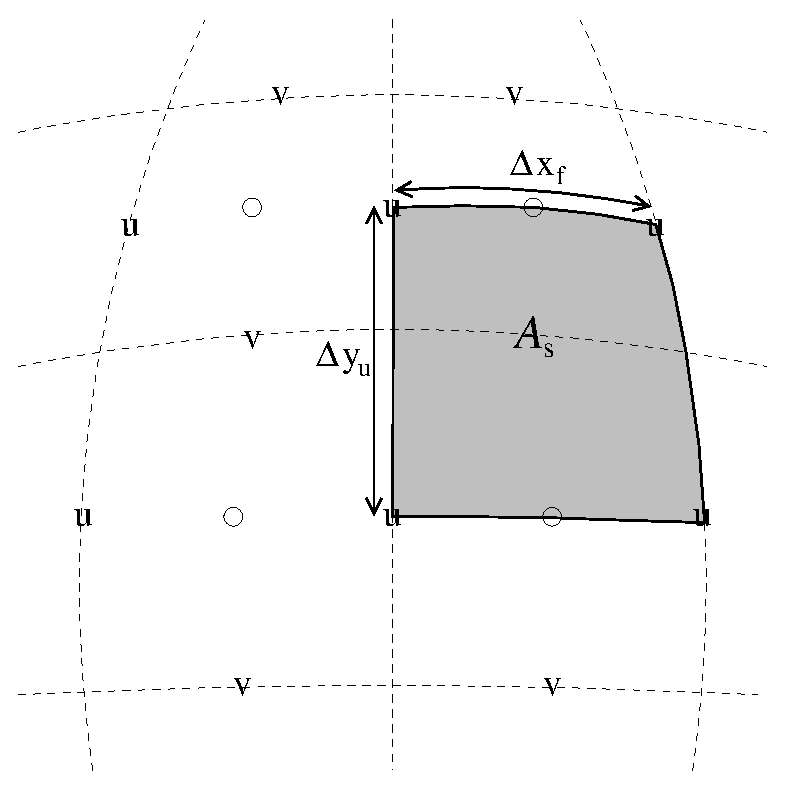
\includegraphics{part2/hgrid-Av.eps}}
\end{tabular}
\end{center}
\caption{
Staggering of horizontal grid descriptors (lengths and areas). The
grid lines indicate the tracer cell boundaries and are the reference
grid for all panels. a) The area of a tracer cell, $A_c$, is bordered
by the lengths $\Delta x_g$ and $\Delta y_g$. b) The area of a
vorticity cell, $A_\zeta$, is bordered by the lengths $\Delta x_c$ and
$\Delta y_c$. c) The area of a u cell, $A_c$, is bordered by the
lengths $\Delta x_v$ and $\Delta y_f$. d) The area of a v cell, $A_c$,
is bordered by the lengths $\Delta x_f$ and $\Delta y_u$.}
\label{fig:hgrid}
\end{figure}

The model domain is decomposed into tiles and within each tile a
quasi-regular grid is used. A tile is the basic unit of domain
decomposition for parallelization but may be used whether parallelized
or not; see section \ref{sect:tiles} for more details. Although the
tiles may be patched together in an unstructured manner
(i.e. irregular or non-tessilating pattern), the interior of tiles is
a structured grid of quadrilateral cells. The horizontal coordinate
system is orthogonal curvilinear meaning we can not necessarily treat
the two horizontal directions as separable. Instead, each cell in the
horizontal grid is described by the length of it's sides and it's
area.

The grid information is quite general and describes any of the
available coordinates systems, cartesian, spherical-polar or
curvilinear. All that is necessary to distinguish between the
coordinate systems is to initialize the grid data (descriptors)
appropriately.

In the following, we refer to the orientation of quantities on the
computational grid using geographic terminology such as points of the
compass.
\marginpar{Caution!}
This is purely for convenience but should note be confused
with the actual geographic orientation of model quantities.

Fig.~\ref{fig:hgrid}a shows the tracer cell (synonymous with the
continuity cell). The length of the southern edge, $\Delta x_g$,
western edge, $\Delta y_g$ and surface area, $A_c$, presented in the
vertical are stored in arrays {\bf DXg}, {\bf DYg} and {\bf rAc}.
\marginpar{$A_c$: {\bf rAc}}
\marginpar{$\Delta x_g$: {\bf DXg}}
\marginpar{$\Delta y_g$: {\bf DYg}}
The ``g'' suffix indicates that the lengths are along the defining
grid boundaries. The ``c'' suffix associates the quantity with the
cell centers. The quantities are staggered in space and the indexing
is such that {\bf DXg(i,j)} is positioned to the south of {\bf
rAc(i,j)} and {\bf DYg(i,j)} positioned to the west.

Fig.~\ref{fig:hgrid}b shows the vorticity cell. The length of the
southern edge, $\Delta x_c$, western edge, $\Delta y_c$ and surface
area, $A_\zeta$, presented in the vertical are stored in arrays {\bf
DXg}, {\bf DYg} and {\bf rAz}.
\marginpar{$A_\zeta$: {\bf rAz}}
\marginpar{$\Delta x_c$: {\bf DXc}}
\marginpar{$\Delta y_c$: {\bf DYc}}
The ``z'' suffix indicates that the lengths are measured between the
cell centers and the ``$\zeta$'' suffix associates points with the
vorticity points. The quantities are staggered in space and the
indexing is such that {\bf DXc(i,j)} is positioned to the north of
{\bf rAc(i,j)} and {\bf DYc(i,j)} positioned to the east.

Fig.~\ref{fig:hgrid}c shows the ``u'' or western (w) cell. The length of
the southern edge, $\Delta x_v$, eastern edge, $\Delta y_f$ and
surface area, $A_w$, presented in the vertical are stored in arrays
{\bf DXv}, {\bf DYf} and {\bf rAw}. 
\marginpar{$A_w$: {\bf rAw}}
\marginpar{$\Delta x_v$: {\bf DXv}}
\marginpar{$\Delta y_f$: {\bf DYf}}
The ``v'' suffix indicates that the length is measured between the
v-points, the ``f'' suffix indicates that the length is measured
between the (tracer) cell faces and the ``w'' suffix associates points
with the u-points (w stands for west). The quantities are staggered in
space and the indexing is such that {\bf DXv(i,j)} is positioned to
the south of {\bf rAw(i,j)} and {\bf DYf(i,j)} positioned to the east.

Fig.~\ref{fig:hgrid}d shows the ``v'' or southern (s) cell. The length of
the northern edge, $\Delta x_f$, western edge, $\Delta y_u$ and
surface area, $A_s$, presented in the vertical are stored in arrays
{\bf DXf}, {\bf DYu} and {\bf rAs}. 
\marginpar{$A_s$: {\bf rAs}}
\marginpar{$\Delta x_f$: {\bf DXf}}
\marginpar{$\Delta y_u$: {\bf DYu}}
The ``u'' suffix indicates that the length is measured between the
u-points, the ``f'' suffix indicates that the length is measured
between the (tracer) cell faces and the ``s'' suffix associates points
with the v-points (s stands for south). The quantities are staggered
in space and the indexing is such that {\bf DXf(i,j)} is positioned to
the north of {\bf rAs(i,j)} and {\bf DYu(i,j)} positioned to the west.

\fbox{ \begin{minipage}{4.75in}
{\em S/R INI\_CARTESIAN\_GRID} ({\em
model/src/ini\_cartesian\_grid.F})

{\em S/R INI\_SPHERICAL\_POLAR\_GRID} ({\em
model/src/ini\_spherical\_polar\_grid.F})

{\em S/R INI\_CURVILINEAR\_GRID} ({\em
model/src/ini\_curvilinear\_grid.F})

$A_c$, $A_\zeta$, $A_w$, $A_s$: {\bf rAc}, {\bf rAz}, {\bf rAw}, {\bf rAs}
({\em GRID.h})

$\Delta x_g$, $\Delta y_g$: {\bf DXg}, {\bf DYg} ({\em GRID.h})

$\Delta x_c$, $\Delta y_c$: {\bf DXc}, {\bf DYc} ({\em GRID.h})

$\Delta x_f$, $\Delta y_f$: {\bf DXf}, {\bf DYf} ({\em GRID.h})

$\Delta x_v$, $\Delta y_u$: {\bf DXv}, {\bf DYu} ({\em GRID.h})

\end{minipage} }

\subsubsection{Reciprocals of horizontal grid descriptors}

%\marginpar{$A_c^{-1}$: {\bf RECIP\_rAc}}
%\marginpar{$A_\zeta^{-1}$: {\bf RECIP\_rAz}}
%\marginpar{$A_w^{-1}$: {\bf RECIP\_rAw}}
%\marginpar{$A_s^{-1}$: {\bf RECIP\_rAs}}
Lengths and areas appear in the denominator of expressions as much as
in the numerator. For efficiency and portability, we pre-calculate the
reciprocal of the horizontal grid quantities so that in-line divisions
can be avoided.

%\marginpar{$\Delta x_g^{-1}$: {\bf RECIP\_DXg}}
%\marginpar{$\Delta y_g^{-1}$: {\bf RECIP\_DYg}}
%\marginpar{$\Delta x_c^{-1}$: {\bf RECIP\_DXc}}
%\marginpar{$\Delta y_c^{-1}$: {\bf RECIP\_DYc}}
%\marginpar{$\Delta x_f^{-1}$: {\bf RECIP\_DXf}}
%\marginpar{$\Delta y_f^{-1}$: {\bf RECIP\_DYf}}
%\marginpar{$\Delta x_v^{-1}$: {\bf RECIP\_DXv}}
%\marginpar{$\Delta y_u^{-1}$: {\bf RECIP\_DYu}}
For each grid descriptor (array) there is a reciprocal named using the
prefix {\bf RECIP\_}. This doubles the amount of storage in {\em
GRID.h} but they are all only 2-D descriptors.

\fbox{ \begin{minipage}{4.75in}
{\em S/R INI\_MASKS\_ETC} ({\em
model/src/ini\_masks\_etc.F})

$A_c^{-1}$: {\bf RECIP\_Ac} ({\em GRID.h})

$A_\zeta^{-1}$: {\bf RECIP\_Az} ({\em GRID.h})

$A_w^{-1}$: {\bf RECIP\_Aw} ({\em GRID.h})

$A_s^{-1}$: {\bf RECIP\_As} ({\em GRID.h})

$\Delta x_g^{-1}$, $\Delta y_g^{-1}$: {\bf RECIP\_DXg}, {\bf RECIP\_DYg} ({\em GRID.h})

$\Delta x_c^{-1}$, $\Delta y_c^{-1}$: {\bf RECIP\_DXc}, {\bf RECIP\_DYc} ({\em GRID.h})

$\Delta x_f^{-1}$, $\Delta y_f^{-1}$: {\bf RECIP\_DXf}, {\bf RECIP\_DYf} ({\em GRID.h})

$\Delta x_v^{-1}$, $\Delta y_u^{-1}$: {\bf RECIP\_DXv}, {\bf RECIP\_DYu} ({\em GRID.h})

\end{minipage} }

\subsubsection{Cartesian coordinates}

Cartesian coordinates are selected when the logical flag {\bf
using\-Cartes\-ianGrid} in namelist {\em PARM04} is set to true. The grid
spacing can be set to uniform via scalars {\bf dXspacing} and {\bf
dYspacing} in namelist {\em PARM04} or to variable resolution by the
vectors {\bf DELX} and {\bf DELY}. Units are normally
meters. Non-dimensional coordinates can be used by interpreting the
gravitational constant as the Rayleigh number.

\subsubsection{Spherical-polar coordinates}

Spherical coordinates are selected when the logical flag {\bf
using\-Spherical\-PolarGrid} in namelist {\em PARM04} is set to true. The
grid spacing can be set to uniform via scalars {\bf dXspacing} and
{\bf dYspacing} in namelist {\em PARM04} or to variable resolution by
the vectors {\bf DELX} and {\bf DELY}. Units of these namelist
variables are alway degrees. The horizontal grid descriptors are
calculated from these namelist variables have units of meters.

\subsubsection{Curvilinear coordinates}

Curvilinear coordinates are selected when the logical flag {\bf
using\-Curvil\-inear\-Grid} in namelist {\em PARM04} is set to true. The
grid spacing can not be set via the namelist. Instead, the grid
descriptors are read from data files, one for each descriptor. As for
other grids, the horizontal grid descriptors have units of meters.


\subsection{Vertical grid}

\begin{figure}
\begin{center}
  \begin{tabular}{cc}
  \raisebox{4in}{a)} \resizebox{!}{4in}{
  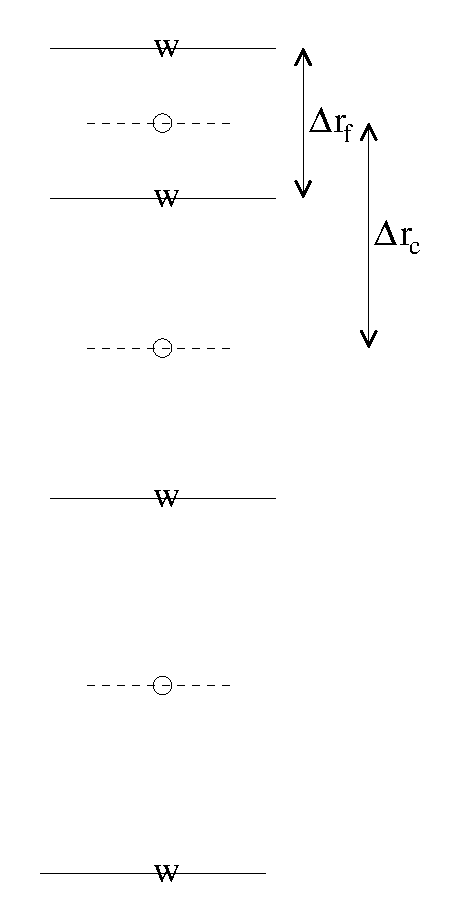
\includegraphics{part2/vgrid-cellcentered.eps}} & \raisebox{4in}{b)}
  \resizebox{!}{4in}{ 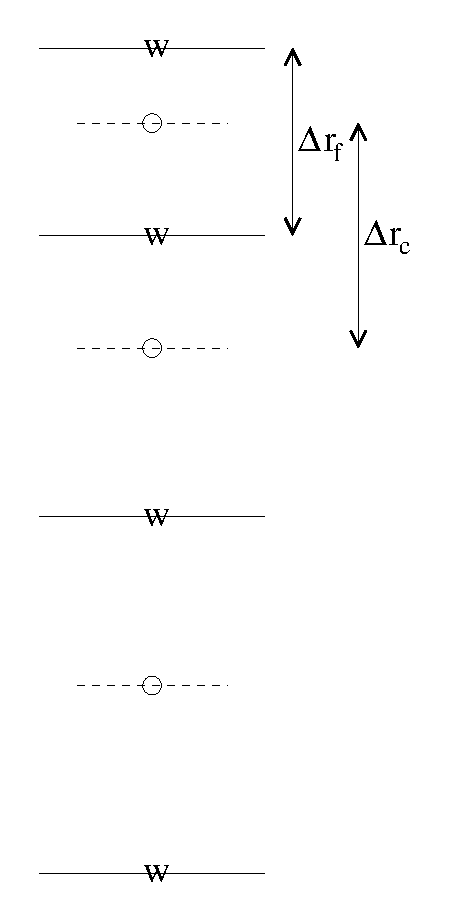
\includegraphics{part2/vgrid-accurate.eps}}
\end{tabular} 
\end{center}
\caption{Two versions of the vertical grid. a) The cell centered
approach where the interface depths are specified and the tracer
points centered in between the interfaces. b) The interface centered
approach where tracer levels are specified and the w-interfaces are
centered in between.}
\label{fig:vgrid}
\end{figure}

As for the horizontal grid, we use the suffixes ``c'' and ``f'' to
indicates faces and centers. Fig.~\ref{fig:vgrid}a shows the default
vertical grid used by the model.
\marginpar{$\Delta r_f$: {\bf DRf}}
\marginpar{$\Delta r_c$: {\bf DRc}}
$\Delta r_f$ is the difference in $r$
(vertical coordinate) between the faces (i.e. $\Delta r_f \equiv -
\delta_k r$ where the minus sign appears due to the convention that the
surface layer has index $k=1$.).

The vertical grid is calculated in subroutine {\em
INI\_VERTICAL\_GRID} and specified via the vector {\bf DELR} in
namelist {\em PARM04}. The units of ``r'' are either meters or Pascals
depending on the isomorphism being used which in turn is dependent
only on the choice of equation of state.

There are alternative namelist vectors {\bf DELZ} and {\bf DELP} which
dictate whether z- or
\marginpar{Caution!}
p- coordinates are to be used but we intend to
phase this out since they are redundant.

The reciprocals $\Delta r_f^{-1}$ and $\Delta r_c^{-1}$ are
pre-calculated (also in subroutine {\em INI\_VERTICAL\_GRID}). All
vertical grid descriptors are stored in common blocks in {\em GRID.h}.

The above grid (Fig.~\ref{fig:vgrid}a) is known as the cell centered
approach because the tracer points are at cell centers; the cell
centers are mid-way between the cell interfaces. An alternative, the
vertex or interface centered approach, is shown in
Fig.~\ref{fig:vgrid}b. Here, the interior interfaces are positioned
mid-way between the tracer nodes (no longer cell centers). This
approach is formally more accurate for evaluation of hydrostatic
pressure and vertical advection but historically the cell centered
approach has been used. An alternative form of subroutine {\em
INI\_VERTICAL\_GRID} is used to select the interface centered approach
but no run time option is currently available.

\fbox{ \begin{minipage}{4.75in}
{\em S/R INI\_VERTICAL\_GRID} ({\em
model/src/ini\_vertical\_grid.F})

$\Delta r_f$: {\bf DRf} ({\em GRID.h})

$\Delta r_c$: {\bf DRc} ({\em GRID.h})

$\Delta r_f^{-1}$: {\bf RECIP\_DRf} ({\em GRID.h})

$\Delta r_c^{-1}$: {\bf RECIP\_DRc} ({\em GRID.h})

\end{minipage} }


\subsection{Topography: partially filled cells}

\begin{figure}
\begin{center}
\resizebox{4.5in}{!}{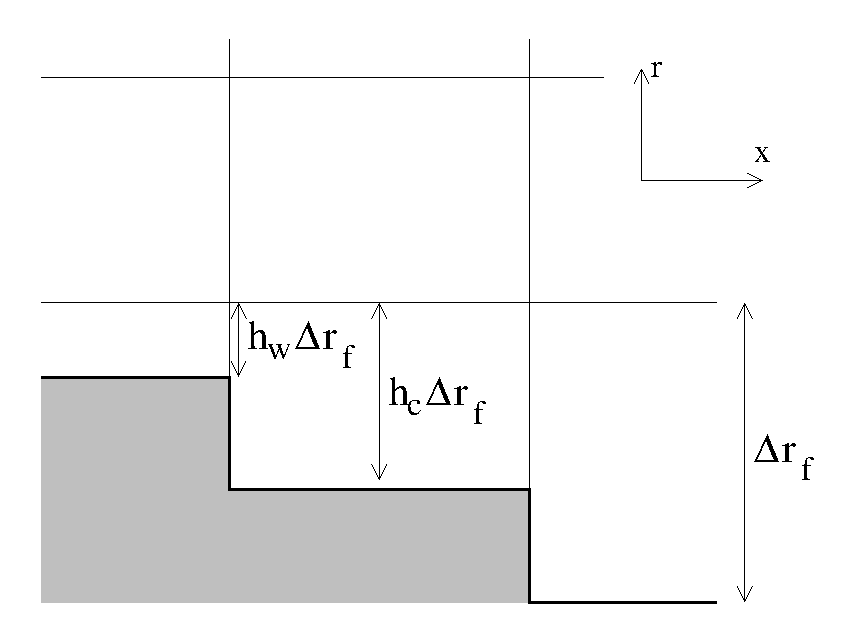
\includegraphics{part2/vgrid-xz.eps}}
\end{center}
\caption{
A schematic of the x-r plane showing the location of the
non-dimensional fractions $h_c$ and $h_w$. The physical thickness of a
tracer cell is given by $h_c(i,j,k) \Delta r_f(k)$ and the physical
thickness of the open side is given by $h_w(i,j,k) \Delta r_f(k)$.}
\label{fig:hfacs}
\end{figure}

\cite{adcroft:97} presented two alternatives to the step-wise finite
difference representation of topography. The method is known to the
engineering community as {\em intersecting boundary method}. It
involves allowing the boundary to intersect a grid of cells thereby
modifying the shape of those cells intersected. We suggested allowing
the topography to take on a piece-wise linear representation (shaved
cells) or a simpler piecewise constant representation (partial step).
Both show dramatic improvements in solution compared to the
traditional full step representation, the piece-wise linear being the
best. However, the storage requirements are excessive so the simpler
piece-wise constant or partial-step method is all that is currently
supported.

Fig.~\ref{fig:hfacs} shows a schematic of the x-r plane indicating how
the thickness of a level is determined at tracer and u points.
\marginpar{$h_c$: {\bf hFacC}}
\marginpar{$h_w$: {\bf hFacW}}
\marginpar{$h_s$: {\bf hFacS}}
The physical thickness of a tracer cell is given by $h_c(i,j,k) \Delta
r_f(k)$ and the physical thickness of the open side is given by
$h_w(i,j,k) \Delta r_f(k)$. Three 3-D descriptors $h_c$, $h_w$ and
$h_s$ are used to describe the geometry: {\bf hFacC}, {\bf hFacW} and
{\bf hFacS} respectively. These are calculated in subroutine {\em
INI\_MASKS\_ETC} along with there reciprocals {\bf RECIP\_hFacC}, {\bf
RECIP\_hFacW} and {\bf RECIP\_hFacS}.

The non-dimensional fractions (or h-facs as we call them) are
calculated from the model depth array and then processed to avoid tiny
volumes. The rule is that if a fraction is less than {\bf hFacMin}
then it is rounded to the nearer of $0$ or {\bf hFacMin} or if the
physical thickness is less than {\bf hFacMinDr} then it is similarly
rounded. The larger of the two methods is used when there is a
conflict. By setting {\bf hFacMinDr} equal to or larger than the
thinnest nominal layers, $\min{(\Delta z_f)}$, but setting {\bf
hFacMin} to some small fraction then the model will only lop thick
layers but retain stability based on the thinnest unlopped thickness;
$\min{(\Delta z_f,\mbox{\bf hFacMinDr})}$.

\fbox{ \begin{minipage}{4.75in}
{\em S/R INI\_MASKS\_ETC} ({\em model/src/ini\_masks\_etc.F})

$h_c$: {\bf hFacC} ({\em GRID.h})

$h_w$: {\bf hFacW} ({\em GRID.h})

$h_s$: {\bf hFacS} ({\em GRID.h})

$h_c^{-1}$: {\bf RECIP\_hFacC} ({\em GRID.h})

$h_w^{-1}$: {\bf RECIP\_hFacW} ({\em GRID.h})

$h_s^{-1}$: {\bf RECIP\_hFacS} ({\em GRID.h})

\end{minipage} }


\section{Continuity and horizontal pressure gradient terms}

The core algorithm is based on the ``C grid'' discretization of the
continuity equation which can be summarized as:
\begin{eqnarray}
\partial_t u + \frac{1}{\Delta x_c} \delta_i \left. \frac{ \partial \Phi}{\partial r}\right|_{s} \eta + \frac{\epsilon_{nh}}{\Delta x_c} \delta_i \Phi_{nh}' & = & G_u - \frac{1}{\Delta x_c} \delta_i \Phi_h' \label{eq:discrete-momu} \\
\partial_t v + \frac{1}{\Delta y_c} \delta_j \left. \frac{ \partial \Phi}{\partial r}\right|_{s} \eta + \frac{\epsilon_{nh}}{\Delta y_c} \delta_j \Phi_{nh}' & = & G_v - \frac{1}{\Delta y_c} \delta_j \Phi_h' \label{eq:discrete-momv} \\
\epsilon_{nh} \left( \partial_t w + \frac{1}{\Delta r_c} \delta_k \Phi_{nh}' \right) & = & \epsilon_{nh} G_w + \overline{b}^k - \frac{1}{\Delta r_c} \delta_k \Phi_{h}' \label{eq:discrete-momw} \\
\delta_i \Delta y_g \Delta r_f h_w u +
\delta_j \Delta x_g \Delta r_f h_s v +
\delta_k {\cal A}_c w & = & {\cal A}_c \delta_k (P-E)_{r=0}
\label{eq:discrete-continuity}
\end{eqnarray}
where the continuity equation has been most naturally discretized by
staggering the three components of velocity as shown in
Fig.~\ref{fig:cgrid3d}. The grid lengths $\Delta x_c$ and $\Delta y_c$
are the lengths between tracer points (cell centers). The grid lengths
$\Delta x_g$, $\Delta y_g$ are the grid lengths between cell
corners. $\Delta r_f$ and $\Delta r_c$ are the distance (in units of
$r$) between level interfaces (w-level) and level centers (tracer
level). The surface area presented in the vertical is denoted ${\cal
A}_c$.  The factors $h_w$ and $h_s$ are non-dimensional fractions
(between 0 and 1) that represent the fraction cell depth that is
``open'' for fluid flow.
\marginpar{$h_w$: {\bf hFacW}}
\marginpar{$h_s$: {\bf hFacS}}

The last equation, the discrete continuity equation, can be summed in
the vertical to yield the free-surface equation:
\begin{equation}
{\cal A}_c \partial_t \eta + \delta_i \sum_k \Delta y_g \Delta r_f h_w
u + \delta_j \sum_k \Delta x_g \Delta r_f h_s v = {\cal
A}_c(P-E)_{r=0} \label{eq:discrete-freesurface}
\end{equation}
The source term $P-E$ on the rhs of continuity accounts for the local
addition of volume due to excess precipitation and run-off over
evaporation and only enters the top-level of the {\em ocean} model.

\section{Hydrostatic balance}

The vertical momentum equation has the hydrostatic or
quasi-hydrostatic balance on the right hand side. This discretization
guarantees that the conversion of potential to kinetic energy as
derived from the buoyancy equation exactly matches the form derived
from the pressure gradient terms when forming the kinetic energy
equation.

In the ocean, using z-coordinates, the hydrostatic balance terms are
discretized:
\begin{equation}
\epsilon_{nh} \partial_t w
+ g \overline{\rho'}^k + \frac{1}{\Delta z} \delta_k \Phi_h' = \ldots
\label{eq:discrete_hydro_ocean}
\end{equation}

In the atmosphere, using p-coordinates, hydrostatic balance is
discretized:
\begin{equation}
\overline{\theta'}^k + \frac{1}{\Delta \Pi} \delta_k \Phi_h' = 0
\label{eq:discrete_hydro_atmos}
\end{equation}
where $\Delta \Pi$ is the difference in Exner function between the
pressure points. The non-hydrostatic equations are not available in
the atmosphere.

The difference in approach between ocean and atmosphere occurs because
of the direct use of the ideal gas equation in forming the potential
energy conversion term $\alpha \omega$. The form of these conversion
terms is discussed at length in \cite{adcroft:02}.

Because of the different representation of hydrostatic balance between
ocean and atmosphere there is no elegant way to represent both systems
using an arbitrary coordinate.

The integration for hydrostatic pressure is made in the positive $r$
direction (increasing k-index). For the ocean, this is from the
free-surface down and for the atmosphere this is from the ground up.

The calculations are made in the subroutine {\em
CALC\_PHI\_HYD}. Inside this routine, one of other of the
atmospheric/oceanic form is selected based on the string variable {\bf
buoyancyRelation}.

